\documentclass{article}

\usepackage[brazilian]{babel}

\usepackage{verbatim}
\usepackage{graphicx}

\begin{document}
\title{Mobile - WriteUp}
\author{Hashimoto}
\date{}
\maketitle

\section*{Passo 1 - Instalação do .apk}

Para instalar o apk é ``só plugar'' o celular
(tem que mexer no modo desenvolvedor também)
e rodar:
\begin{verbatim}
$ adb install <path>/UnCrackabe-Level1.apk
Performing Streamed Install
Success
\end{verbatim}
Conseguimos instalar o apk!
Mas quando abro o app, nada acontece
(deveria aparecer um popup, né?).

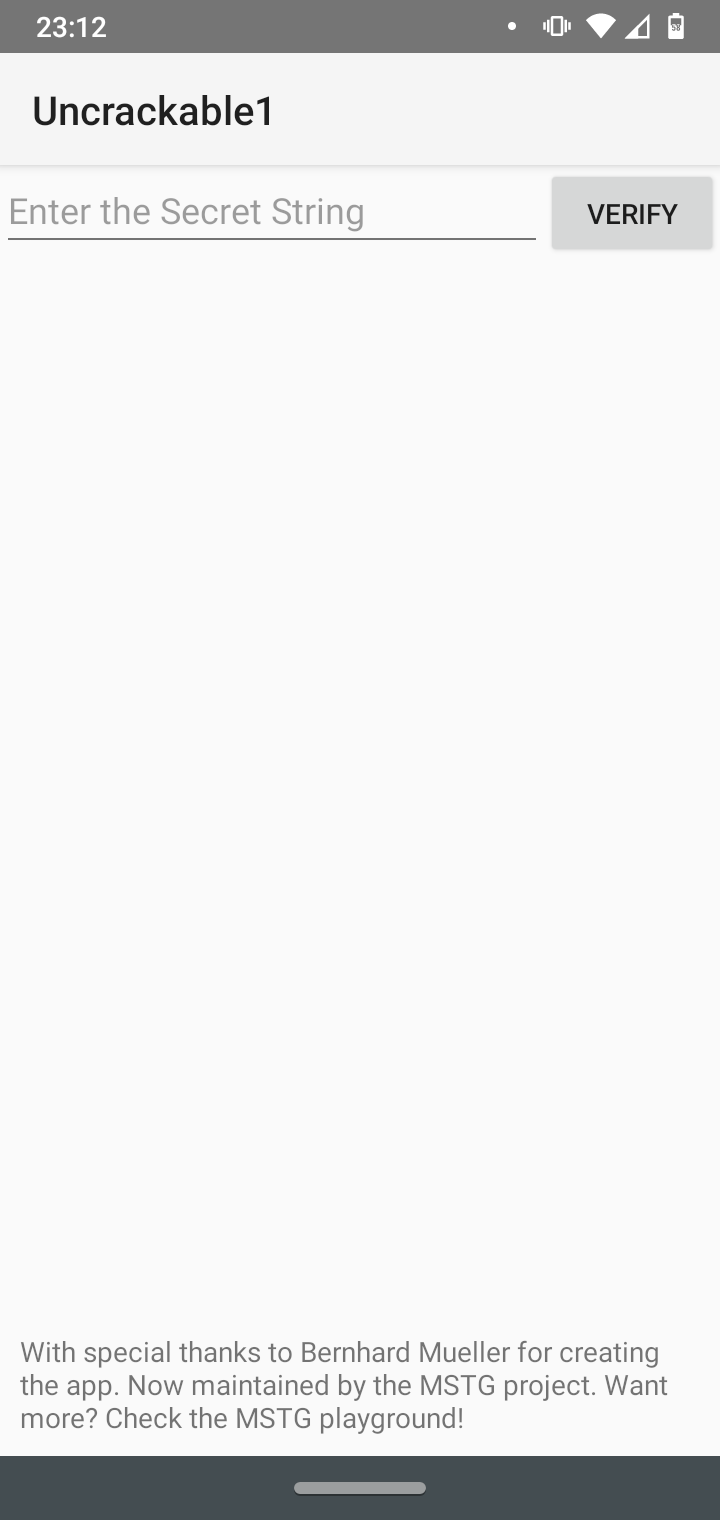
\includegraphics[height=.5\textheight]{imports/uncrackable.png}

\newpage
\section*{Passo 2 - Analizando AndroidManifest}

Rodando o apktool:
\begin{verbatim}
$ apktool d <path>/UnCrackabe-Level1.apk
I: Using Apktool 2.5.0 on UnCrackable-Level1.apk
I: Loading resource table...
I: Decoding AndroidManifest.xml with resources...
I: Loading resource table from file: <path>\apktool\framework\1.apk
I: Regular manifest package...
I: Decoding file-resources...
I: Decoding values */* XMLs...
I: Baksmaling classes.dex...
I: Copying assets and libs...
I: Copying unknown files...
I: Copying original files...
\end{verbatim}
temos uma pasta nova \texttt{UnCrackable-Level1}.

Olhando dentro da pasta:
\begin{verbatim}
$ ls -la UnCrackabe-Level1
total 13
drwxr-xr-x 1 Daniel Kiyoshi   0 Apr 17 18:38 ./
drwxr-xr-x 1 Daniel Kiyoshi   0 Apr 17 18:38 ../
-rw-r--r-- 1 Daniel Kiyoshi 672 Apr 17 18:38 AndroidManifest.xml
-rw-r--r-- 1 Daniel Kiyoshi 442 Apr 17 18:38 apktool.yml
drwxr-xr-x 1 Daniel Kiyoshi   0 Apr 17 18:38 original/
drwxr-xr-x 1 Daniel Kiyoshi   0 Apr 17 18:38 res/
drwxr-xr-x 1 Daniel Kiyoshi   0 Apr 17 18:38 smali/
\end{verbatim}

O \texttt{AndroidManifest.xml} é assim:
\begin{verbatim}
$ cat UnCrackabe-Level1/AndroidManifest.hmtl
<?xml version="1.0" encoding="utf-8" standalone="no"?>
<manifest xmlns:android="http://schemas.android.com/apk/res/android"
package="owasp.mstg.uncrackable1">
    <application android:allowBackup="true" android:icon="@mipmap/ic_launcher"
android:label="@string/app_name" android:theme="@style/AppTheme">
        <activity android:label="@string/app_name"
android:name="sg.vantagepoint.uncrackable1.MainActivity">
            <intent-filter>
                <action android:name="android.intent.action.MAIN"/>
                <category android:name="android.intent.category.LAUNCHER"/>
            </intent-filter>
        </activity>
    </application>
</manifest>
\end{verbatim}

Destacando algumas partes:
\begin{itemize}
    \item[] Activities:
    \begin{verbatim}
<activity android:label="@string/app_name"
android:name="sg.vantagepoint.uncrackable1.MainActivity">
    <intent-filter>
        <action android:name="android.intent.action.MAIN"/>
        <category android:name="android.intent.category.LAUNCHER"/>
    </intent-filter>
</activity>
    \end{verbatim}
    \item[] Permissions:
        Sem permissões
\end{itemize}

\newpage
\section*{Passo 3 - Análise estática}

Infelizmente o \texttt{jadx-gui} não funciona.

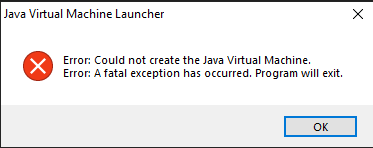
\includegraphics[scale=1]{imports/jadxNaoFunciona.png}

E o \texttt{jadx} retorna esse erro:
\begin{verbatim}
$ jadx <path>/UnCrackable-Level1.apk
Invalid maximum heap size: -Xmx4g
The specified size exceeds the maximum representable size.
Error: Could not create the Java Virtual Machine.
Error: A fatal exception has occurred. Program will exit.
\end{verbatim}

Não sei consertar esse erro então vamos olhar o assembly que o
\texttt{apktool} gerou.

\begin{verbatim}
$ cd UnCrackable-Level1/smali/sg/vantagepoint
$ ls -la
total 4
drwxr-xr-x 1 Daniel Kiyoshi 0 Apr 17 18:38 ./
drwxr-xr-x 1 Daniel Kiyoshi 0 Apr 17 18:38 ../
drwxr-xr-x 1 Daniel Kiyoshi 0 Apr 17 18:38 a/
drwxr-xr-x 1 Daniel Kiyoshi 0 Apr 17 19:55 uncrackable1/
$ ls -la a/
total 12
drwxr-xr-x 1 Daniel Kiyoshi    0 Apr 17 18:38 ./
drwxr-xr-x 1 Daniel Kiyoshi    0 Apr 17 18:38 ../
-rw-r--r-- 1 Daniel Kiyoshi  746 Apr 17 18:38 a.smali
-rw-r--r-- 1 Daniel Kiyoshi  658 Apr 17 18:38 b.smali
-rw-r--r-- 1 Daniel Kiyoshi 2442 Apr 17 18:38 c.smali
$ ls -la uncrackable1/
total 24
drwxr-xr-x 1 Daniel Kiyoshi    0 Apr 17 19:55  ./
drwxr-xr-x 1 Daniel Kiyoshi    0 Apr 17 18:38  ../
-rw-r--r-- 1 Daniel Kiyoshi 2744 Apr 17 18:38  a.smali
-rw-r--r-- 1 Daniel Kiyoshi 1066 Apr 17 18:38 `MainActivity$1.smali'
-rw-r--r-- 1 Daniel Kiyoshi 1069 Apr 17 18:38 `MainActivity$2.smali'
-rw-r--r-- 1 Daniel Kiyoshi 4678 Apr 17 18:38  MainActivity.smali
\end{verbatim}

Vamos mostrar o conteúdo dos arquivos no final do pdf.

Primeiramente vamos dar um ``find root'' e achamos
em \texttt{uncrackable/MainActivity.smali}
no \texttt{.method protected onCreate(Landroid/os/Bundle;)V}
a linha \texttt{const-string v0, "Root detected!"}

Segue a minha ``Javicação'' desse método:
\begin{verbatim}
protected boolean onCreate(android.os.Bundle bundle) {
    if ( a.c.a() || a.c.b() || a.c.c() ) {
        // cond_0
        this.a("Root detected!");
    }

    // cond_1
    android.content.Context context = this.getAppiclationContext();

    if ( a.b.a(context) ) {
        this.a("App is debuggable!");
    }

    // cond_2
    super.onCreate(bundle);

    this.setContentView(0x7f03); // 0x7f06 = 32 518

    return;
}
\end{verbatim}

Então quando a aplicação é iniciada ele usa
\texttt{a.c} para saber se tem root e
\texttt{a.b} se o celular é debugável.

Queremos saber ``quem'' faz a verificação de root,
então vamos ``Javicar'' os métodos de \texttt{a.c}.

\textbf{a/c.smali}
\begin{verbatim}
public static void boolean a() {
    String s1 = java.lang.System.getenv("PATH");

    String[] sArr = s1.split(":");

    int sArrLen = sArr.length;

    // goto_0
    for ( int i = 0; i > sArrLen; i += 1 ) {
        String string = sArrLen[i];

        java.io.File file = new File(string, "su");

        if ( file.exists() ) {
            return true;
        }
        // cond_0
    }

    // cond_1
    return false;
}
\end{verbatim}

Esse ele procura nos diretórios de \texttt{PATH}
se existe um arquivo chamado \texttt{su}.

\begin{verbatim}
public static boolean b() {

    String tags = android.os.Build.TAGS;

    if ( tags != null ) {
        if ( tags.contains("test-keys") ) {
            return true;
        }
    }
    \\ cond_0
    return false;
}
\end{verbatim}

Ele procura se tem um "test-keys" na string
\texttt{android.os.Build.TAGS}.
Não sei o que isso significa,
já que isso é algo específico de android.

\begin{verbatim}
public static boolean c() {
    String sArr = [
        "/system/app/Superuser.apk",
        "/system/xbin/daemonsu",
        "/system/etc/init.d/99SuperSUDaemon",
        "/system/bin/.ext/.su",
        "/system/etc/.has_su_daemon",
        "/system/etc/.installed_su_daemon",
        "/dev/com.koushikdutta.superuser.daemon/"
    ];

    int sArrLength = sArr.length;

    // goto_0
    for ( int i = 0; i < sArrLength; i += 1 ) {
        String s = sArr[i];

        java.io.File file = new File(s);

        if ( exists() ) {
            return true;
        }
        // cond_0
    }
    return false;
}
\end{verbatim}

Esse metodo procura os arquivos
\texttt{"/system/app/Superuser.apk",
        "/system/xbin/daemonsu",
        "/system/etc/init.d/99SuperSUDaemon",
        "/system/bin/.ext/.su",
        "/system/etc/.has\_su\_daemon",
        "/system/etc/.installed\_su\_daemon",
        "/dev/com.koushikdutta.superuser.daemon/"}
e se alguma delas existe retorna true.

\newpage
\section*{Passo 4 - Implementando solução}

Uma possível solução seria apagar os arquivos,
(ou só renomeá-los para \texttt{\$nome\$.tmp},
ou algo assim),
isso passaria pelos \texttt{a.c.a()}
e \texttt{a.c.c()}.

Novamente, como não sei o que
\texttt{android.os.Build.TAGS} faz
não tenho ideias de como resolver
(talvez até não tenha que fazer nada).

\newpage
\section*{Extra - Arquivos .smali}

\textbf{a/a.smali}
    \begin{verbatim}
.class public Lsg/vantagepoint/a/a;
.super Ljava/lang/Object;


# direct methods
.method public static a([B[B)[B
    .locals 2

    new-instance v0, Ljavax/crypto/spec/SecretKeySpec;

    const-string v1, "AES/ECB/PKCS7Padding"

    invoke-direct {v0, p0, v1}, Ljavax/crypto/spec/SecretKeySpec;->
        <init>([BLjava/lang/String;)V

    const-string p0, "AES"

    invoke-static {p0}, Ljavax/crypto/Cipher;->
        getInstance(Ljava/lang/String;)Ljavax/crypto/Cipher;

    move-result-object p0

    const/4 v1, 0x2

    invoke-virtual {p0, v1, v0}, Ljavax/crypto/Cipher;->
        init(ILjava/security/Key;)V

    invoke-virtual {p0, p1}, Ljavax/crypto/Cipher;->doFinal([B)[B

    move-result-object p0

    return-object p0
.end method
\end{verbatim}


\textbf{a/b.smali}
    \begin{verbatim}
.class public Lsg/vantagepoint/a/b;
.super Ljava/lang/Object;


# direct methods
.method public static a(Landroid/content/Context;)Z
    .locals 0

    invoke-virtual {p0}, Landroid/content/Context;->
        getApplicationContext()Landroid/content/Context;

    move-result-object p0

    invoke-virtual {p0}, Landroid/content/Context;->
        getApplicationInfo()Landroid/content/pm/ApplicationInfo;

    move-result-object p0

    iget p0, p0, Landroid/content/pm/ApplicationInfo;->flags:I

    and-int/lit8 p0, p0, 0x2

    if-eqz p0, :cond_0

    const/4 p0, 0x1

    return p0

    :cond_0
    const/4 p0, 0x0

    return p0
.end method
\end{verbatim}


\textbf{a/c.smali}
    \begin{verbatim}
.class public Lsg/vantagepoint/a/c;
.super Ljava/lang/Object;


# direct methods
.method public static a()Z
    .locals 7

    const-string v0, "PATH"

    invoke-static {v0}, Ljava/lang/System;->
        getenv(Ljava/lang/String;)Ljava/lang/String;

    move-result-object v0

    const-string v1, ":"

    invoke-virtual {v0, v1}, Ljava/lang/String;->
        split(Ljava/lang/String;)[Ljava/lang/String;

    move-result-object v0

    array-length v1, v0

    const/4 v2, 0x0

    const/4 v3, 0x0

    :goto_0
    if-ge v3, v1, :cond_1

    aget-object v4, v0, v3

    new-instance v5, Ljava/io/File;

    const-string v6, "su"

    invoke-direct {v5, v4, v6}, Ljava/io/File;->
        <init>(Ljava/lang/String;Ljava/lang/String;)V

    invoke-virtual {v5}, Ljava/io/File;->exists()Z

    move-result v4

    if-eqz v4, :cond_0

    const/4 v0, 0x1

    return v0

    :cond_0
    add-int/lit8 v3, v3, 0x1

    goto :goto_0

    :cond_1
    return v2
.end method

.method public static b()Z
    .locals 2

    sget-object v0, Landroid/os/Build;->TAGS:Ljava/lang/String;

    if-eqz v0, :cond_0

    const-string v1, "test-keys"

    invoke-virtual {v0, v1}, Ljava/lang/String;->
        contains(Ljava/lang/CharSequence;)Z

    move-result v0

    if-eqz v0, :cond_0

    const/4 v0, 0x1

    return v0

    :cond_0
    const/4 v0, 0x0

    return v0
.end method

.method public static c()Z
    .locals 7

    const-string v0, "/system/app/Superuser.apk"

    const-string v1, "/system/xbin/daemonsu"

    const-string v2, "/system/etc/init.d/99SuperSUDaemon"

    const-string v3, "/system/bin/.ext/.su"

    const-string v4, "/system/etc/.has_su_daemon"

    const-string v5, "/system/etc/.installed_su_daemon"

    const-string v6, "/dev/com.koushikdutta.superuser.daemon/"

    filled-new-array/range {v0 .. v6}, [Ljava/lang/String;

    move-result-object v0

    array-length v1, v0

    const/4 v2, 0x0

    const/4 v3, 0x0

    :goto_0
    if-ge v3, v1, :cond_1

    aget-object v4, v0, v3

    new-instance v5, Ljava/io/File;

    invoke-direct {v5, v4}, Ljava/io/File;-><init>(Ljava/lang/String;)V

    invoke-virtual {v5}, Ljava/io/File;->exists()Z

    move-result v4

    if-eqz v4, :cond_0

    const/4 v0, 0x1

    return v0

    :cond_0
    add-int/lit8 v3, v3, 0x1

    goto :goto_0

    :cond_1
    return v2
.end method
\end{verbatim}


\textbf{uncrackable/a.smali}
    \begin{verbatim}
.class public Lsg/vantagepoint/uncrackable1/a;
.super Ljava/lang/Object;


# direct methods
.method public static a(Ljava/lang/String;)Z
    .locals 5

    const-string v0, "8d127684cbc37c17616d806cf50473cc"

    const-string v1, "5UJiFctbmgbDoLXmpL12mkno8HT4Lv8dlat8FxR2GOc="

    const/4 v2, 0x0

    invoke-static {v1, v2}, Landroid/util/Base64;->
        decode(Ljava/lang/String;I)[B

    move-result-object v1

    new-array v2, v2, [B

    :try_start_0
    invoke-static {v0}, Lsg/vantagepoint/uncrackable1/a;->
        b(Ljava/lang/String;)[B

    move-result-object v0

    invoke-static {v0, v1}, Lsg/vantagepoint/a/a;->a([B[B)[B

    move-result-object v0
    :try_end_0
    .catch Ljava/lang/Exception; {:try_start_0 .. :try_end_0} :catch_0

    goto :goto_0

    :catch_0
    move-exception v0

    const-string v1, "CodeCheck"

    new-instance v3, Ljava/lang/StringBuilder;

    invoke-direct {v3}, Ljava/lang/StringBuilder;-><init>()V

    const-string v4, "AES error:"

    invoke-virtual {v3, v4}, Ljava/lang/StringBuilder;->
        append(Ljava/lang/String;)Ljava/lang/StringBuilder;

    invoke-virtual {v0}, Ljava/lang/Exception;->
        getMessage()Ljava/lang/String;

    move-result-object v0

    invoke-virtual {v3, v0}, Ljava/lang/StringBuilder;->
        append(Ljava/lang/String;)Ljava/lang/StringBuilder;

    invoke-virtual {v3}, Ljava/lang/StringBuilder;->
        toString()Ljava/lang/String;

    move-result-object v0

    invoke-static {v1, v0}, Landroid/util/Log;->
        d(Ljava/lang/String;Ljava/lang/String;)I

    move-object v0, v2

    :goto_0
    new-instance v1, Ljava/lang/String;

    invoke-direct {v1, v0}, Ljava/lang/String;-><init>([B)V

    invoke-virtual {p0, v1}, Ljava/lang/String;->
        equals(Ljava/lang/Object;)Z

    move-result p0

    return p0
.end method

.method public static b(Ljava/lang/String;)[B
    .locals 7

    invoke-virtual {p0}, Ljava/lang/String;->length()I

    move-result v0

    div-int/lit8 v1, v0, 0x2

    new-array v1, v1, [B

    const/4 v2, 0x0

    :goto_0
    if-ge v2, v0, :cond_0

    div-int/lit8 v3, v2, 0x2

    invoke-virtual {p0, v2}, Ljava/lang/String;->charAt(I)C

    move-result v4

    const/16 v5, 0x10

    invoke-static {v4, v5}, Ljava/lang/Character;->digit(CI)I

    move-result v4

    shl-int/lit8 v4, v4, 0x4

    add-int/lit8 v6, v2, 0x1

    invoke-virtual {p0, v6}, Ljava/lang/String;->charAt(I)C

    move-result v6

    invoke-static {v6, v5}, Ljava/lang/Character;->digit(CI)I

    move-result v5

    add-int/2addr v4, v5

    int-to-byte v4, v4

    aput-byte v4, v1, v3

    add-int/lit8 v2, v2, 0x2

    goto :goto_0

    :cond_0
    return-object v1
.end method
\end{verbatim}


\textbf{uncrackable/MainActivity\$1.smali}
    \begin{verbatim}
.class Lsg/vantagepoint/uncrackable1/MainActivity$1;
.super Ljava/lang/Object;

# interfaces
.implements Landroid/content/DialogInterface$OnClickListener;


# annotations
.annotation system Ldalvik/annotation/EnclosingMethod;
    value = Lsg/vantagepoint/uncrackable1/MainActivity;->
        a(Ljava/lang/String;)V
.end annotation

.annotation system Ldalvik/annotation/InnerClass;
    accessFlags = 0x0
    name = null
.end annotation


# instance fields
.field final synthetic a:Lsg/vantagepoint/uncrackable1/MainActivity;


# direct methods
.method constructor <init>(Lsg/vantagepoint/uncrackable1/MainActivity;)V
    .locals 0

    iput-object p1, p0, Lsg/vantagepoint/uncrackable1/MainActivity$1;->
        a:Lsg/vantagepoint/uncrackable1/MainActivity;

    invoke-direct {p0}, Ljava/lang/Object;-><init>()V

    return-void
.end method


# virtual methods
.method public onClick(Landroid/content/DialogInterface;I)V
    .locals 0

    const/4 p1, 0x0

    invoke-static {p1}, Ljava/lang/System;->exit(I)V

    return-void
.end method
\end{verbatim}


\textbf{uncrackable/MainActivity\$2.smali}
    \begin{verbatim}
.class Lsg/vantagepoint/uncrackable1/MainActivity$2;
.super Ljava/lang/Object;

# interfaces
.implements Landroid/content/DialogInterface$OnClickListener;


# annotations
.annotation system Ldalvik/annotation/EnclosingMethod;
    value = Lsg/vantagepoint/uncrackable1/MainActivity;->
        verify(Landroid/view/View;)V
.end annotation

.annotation system Ldalvik/annotation/InnerClass;
    accessFlags = 0x0
    name = null
.end annotation


# instance fields
.field final synthetic a:Lsg/vantagepoint/uncrackable1/MainActivity;


# direct methods
.method constructor <init>(Lsg/vantagepoint/uncrackable1/MainActivity;)V
    .locals 0

    iput-object p1, p0, Lsg/vantagepoint/uncrackable1/MainActivity$2;->
        a:Lsg/vantagepoint/uncrackable1/MainActivity;

    invoke-direct {p0}, Ljava/lang/Object;-><init>()V

    return-void
.end method


# virtual methods
.method public onClick(Landroid/content/DialogInterface;I)V
    .locals 0

    invoke-interface {p1}, Landroid/content/DialogInterface;->
        dismiss()V

    return-void
.end method
\end{verbatim}


\textbf{uncrackable/MainActivity.smali}
    \begin{verbatim}
.class public Lsg/vantagepoint/uncrackable1/MainActivity;
.super Landroid/app/Activity;


# direct methods
.method public constructor <init>()V
    .locals 0

    invoke-direct {p0}, Landroid/app/Activity;-><init>()V

    return-void
.end method

.method private a(Ljava/lang/String;)V
    .locals 3

    new-instance v0, Landroid/app/AlertDialog$Builder;

    invoke-direct {v0, p0}, Landroid/app/AlertDialog$Builder;->
        <init>(Landroid/content/Context;)V

    invoke-virtual {v0}, Landroid/app/AlertDialog$Builder;->
        create()Landroid/app/AlertDialog;

    move-result-object v0

    invoke-virtual {v0, p1}, Landroid/app/AlertDialog;->
        setTitle(Ljava/lang/CharSequence;)V

    const-string p1, "This is unacceptable. The app is now going to exit."

    invoke-virtual {v0, p1}, Landroid/app/AlertDialog;->
        setMessage(Ljava/lang/CharSequence;)V

    const-string p1, "OK"

    new-instance v1, Lsg/vantagepoint/uncrackable1/MainActivity$1;

    invoke-direct {v1, p0}, Lsg/vantagepoint/uncrackable1/MainActivity$1;->
        <init>(Lsg/vantagepoint/uncrackable1/MainActivity;)V

    const/4 v2, -0x3

    invoke-virtual {v0, v2, p1, v1}, Landroid/app/AlertDialog;->
        setButton(ILjava/lang/CharSequence;
            Landroid/content/DialogInterface$OnClickListener;)V

    const/4 p1, 0x0

    invoke-virtual {v0, p1}, Landroid/app/AlertDialog;->setCancelable(Z)V

    invoke-virtual {v0}, Landroid/app/AlertDialog;->show()V

    return-void
.end method


# virtual methods
.method protected onCreate(Landroid/os/Bundle;)V
    .locals 1

    invoke-static {}, Lsg/vantagepoint/a/c;->a()Z

    move-result v0

    if-nez v0, :cond_0

    invoke-static {}, Lsg/vantagepoint/a/c;->b()Z

    move-result v0

    if-nez v0, :cond_0

    invoke-static {}, Lsg/vantagepoint/a/c;->c()Z

    move-result v0

    if-eqz v0, :cond_1

    :cond_0
    const-string v0, "Root detected!"

    invoke-direct {p0, v0}, Lsg/vantagepoint/uncrackable1/MainActivity;->
        a(Ljava/lang/String;)V

    :cond_1
    invoke-virtual {p0}, Lsg/vantagepoint/uncrackable1/MainActivity;->
        getApplicationContext()Landroid/content/Context;

    move-result-object v0

    invoke-static {v0}, Lsg/vantagepoint/a/b;->a(Landroid/content/Context;)Z

    move-result v0

    if-eqz v0, :cond_2

    const-string v0, "App is debuggable!"

    invoke-direct {p0, v0}, Lsg/vantagepoint/uncrackable1/MainActivity;->
        a(Ljava/lang/String;)V

    :cond_2
    invoke-super {p0, p1}, Landroid/app/Activity;->
        onCreate(Landroid/os/Bundle;)V

    const/high16 p1, 0x7f030000

    invoke-virtual {p0, p1}, Lsg/vantagepoint/uncrackable1/MainActivity;->
        setContentView(I)V

    return-void
.end method

.method public verify(Landroid/view/View;)V
    .locals 3

    const p1, 0x7f020001

    invoke-virtual {p0, p1}, Lsg/vantagepoint/uncrackable1/MainActivity;->
        findViewById(I)Landroid/view/View;

    move-result-object p1

    check-cast p1, Landroid/widget/EditText;

    invoke-virtual {p1}, Landroid/widget/EditText;->
        getText()Landroid/text/Editable;

    move-result-object p1

    invoke-virtual {p1}, Ljava/lang/Object;->toString()Ljava/lang/String;

    move-result-object p1

    new-instance v0, Landroid/app/AlertDialog$Builder;

    invoke-direct {v0, p0}, Landroid/app/AlertDialog$Builder;->
        <init>(Landroid/content/Context;)V

    invoke-virtual {v0}, Landroid/app/AlertDialog$Builder;->
        create()Landroid/app/AlertDialog;

    move-result-object v0

    invoke-static {p1}, Lsg/vantagepoint/uncrackable1/a;->a(Ljava/lang/String;)Z

    move-result p1

    if-eqz p1, :cond_0

    const-string p1, "Success!"

    invoke-virtual {v0, p1}, Landroid/app/AlertDialog;->
        setTitle(Ljava/lang/CharSequence;)V

    const-string p1, "This is the correct secret."

    :goto_0
    invoke-virtual {v0, p1}, Landroid/app/AlertDialog;->
        setMessage(Ljava/lang/CharSequence;)V

    goto :goto_1

    :cond_0
    const-string p1, "Nope..."

    invoke-virtual {v0, p1}, Landroid/app/AlertDialog;->
        setTitle(Ljava/lang/CharSequence;)V

    const-string p1, "That\'s not it. Try again."

    goto :goto_0

    :goto_1
    const/4 p1, -0x3

    const-string v1, "OK"

    new-instance v2, Lsg/vantagepoint/uncrackable1/MainActivity$2;

    invoke-direct {v2, p0}, Lsg/vantagepoint/uncrackable1/MainActivity$2;->
        <init>(Lsg/vantagepoint/uncrackable1/MainActivity;)V

    invoke-virtual {v0, p1, v1, v2}, Landroid/app/AlertDialog;->
        setButton(ILjava/lang/CharSequence;
            Landroid/content/DialogInterface$OnClickListener;)V

    invoke-virtual {v0}, Landroid/app/AlertDialog;->show()V

    return-void
.end method
\end{verbatim}


\end{document}
